\section{Auswertung}
\label{sec:Auswertung}

Für die Auswertung wird die \texttt{Python}-Bibliothek \texttt{numpy} \cite{numpy} benutzt. Die Fits entstehen mit \texttt{curve\_fit} aus \texttt{scipy.optimize} \cite{scipy}.
Die Fehlerrechnung wird mit \texttt{uncertainties} \cite{uncertainties} durchgeführt. Plots entstehen mit \texttt{matplotlib.pyplot} \cite{matplotlib}. \\
Der Mittelwert $\bar{x}$ von $N$ gemessenen Werten $a$ bestimmt sich über
\begin{equation}
    \bar{x} = \frac{1}{N} \sum^N_{i=1} a_i,
    \label{eq:mittelwerte}
\end{equation}
der Fehler des Mittelwertes über
\begin{equation}
    \Delta x = \sqrt{\frac{1}{N \cdot (N-1)} \sum^N_{i=1}(a_i - \bar{x})}.
    \label{eq:mittelwerte_fehler}
\end{equation}
Die Gaußsche Fehlerfortpflanzung für eine berechnete Größe $f$ lautet
\begin{equation}
    \Delta f = \sqrt{ \sum^N_{i=1} \left( \frac{delta f}{\delta x_i}\right)^2 \cdot (\Delta x_i)^2}.
\end{equation}
Prozentuale Abweichungen werden mit
\begin{equation}
    \Delta x = \left|\frac{x - a}{a}\right|
\end{equation}
berechnet, wobei $a$ ein Vergleichswert und $x$ der erhaltene Wert ist.
\subsection{Europium-152}

Die Messung von Europium ergibt folgendes Spektrum.

\begin{figure}[H]
    \centering
    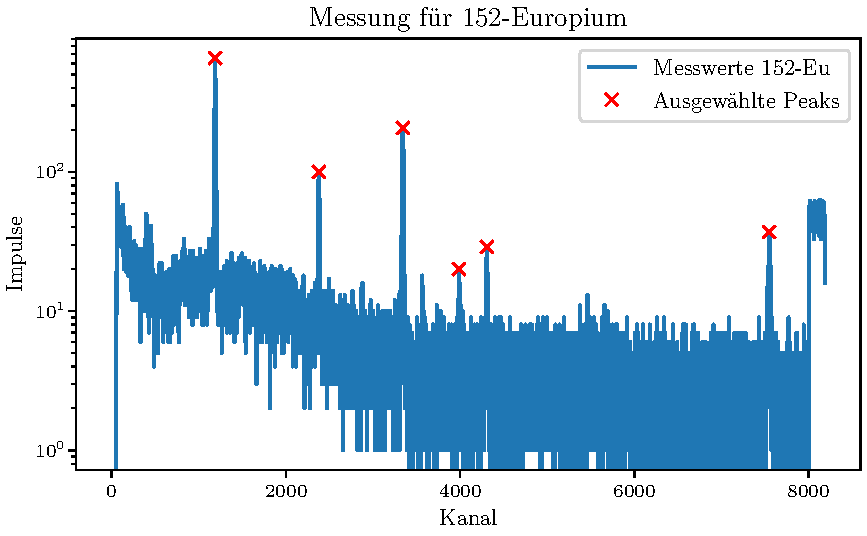
\includegraphics[width=\textwidth]{plots/Europium.pdf}
    \caption{Die Messung für Europium mit ausgewählten, markierten Peaks.}
    \label{fig:Europium}
\end{figure}

Die Kanäle können anhand ihrer relativen Lage und ihrer Impulsmenge bestimmten bekannten Energien zugeordnet werden. Die Linieninhalte, also die Menge an Impulsen, wird hier lediglich als eine Summe über alle beitragenden Kanäle berechnet.
Eine genauere Alternative wäre ein numerisches Integral.
%%%%%% CITE LNHB

\begin{table}[H]
    \centering
    \caption{Europium-Peaks, vgl. \autoref{tab:LNHB_Eu152}}
    \label{tab:europiumpeaks}
    \begin{tabular}{c c c c}
        \toprule
        {Energie ($\si{\kilo\electronvolt}$)} & {Wahrscheinlichkeit in $\%$} & {Kanalnr.} & {Linieninhalt} \\
        \midrule
        121,78 &  28,6 & 1188 & 10375 \pm \, 101\\
        244,70 &  7,6  & 2380 & 1905  \pm \, 43\\
        344,30 &  26,5 & 3344 & 4081  \pm \, 63\\
        411,12 &  2,2  & 3986 & 406   \pm \, 20\\
        443,96 &  3,1  & 4308 & 488   \pm \, 22\\
        778,90 &  12,9 & 7550 & 841   \pm \, 29\\
        \bottomrule
    \end{tabular}
\end{table}

Das Verhältnis von Kanälen zu Energien kann linear beschrieben werden und gibt dann eine Funktion, mit der die Kanalnummer in eine Energie übersetzt werden kann.

\begin{figure}[H]
    \centering
    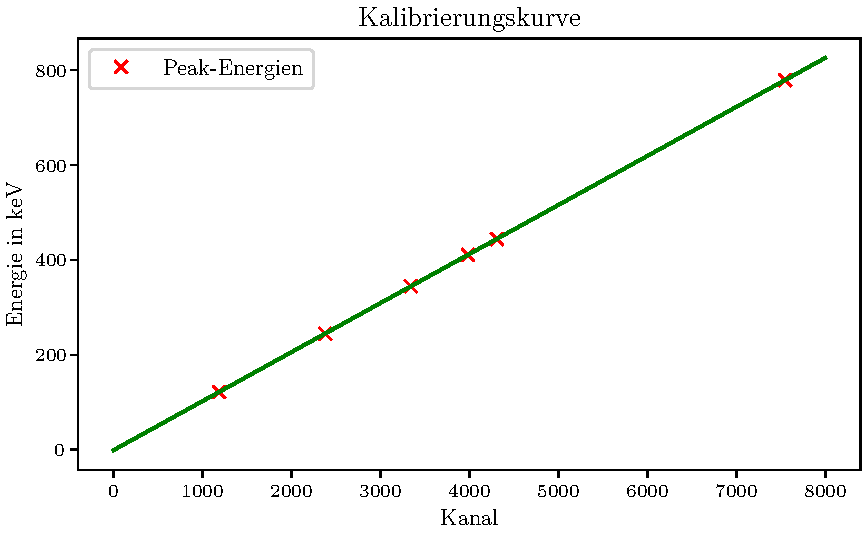
\includegraphics[width=\textwidth]{plots/EuKalibrierung.pdf}
    \caption{Energie und Kanalnummer, linear gefittet.}
    \label{fig:kalibrierung}
\end{figure}

Die Fitfunktion lautet
\begin{equation}
    E(K) = (0,103304 \pm 0,000044) \, \si{\kilo\electronvolt} \, \cdot K - (0,903881 \pm 0,188430) \, \si{\kilo\electronvolt}
    \label{eq:kanalenergie}
\end{equation}

Die Anfangsaktivität $A_0$ am 1. Oktober 2000 beträgt $A_0 = (4130 \pm 60) \, \si{\becquerel}$. Europium-152 hat eine Halbwertszeit von ungefähr $\num{13,53}$ Jahren \cite{hwz-eu}.
Die Durchführung fand ungefähr $\num{24,11}$ Jahre später statt.
Die daraus errechnete Aktivität beträgt
\begin{equation}
    A = (1202 \pm 17) \, \si{\becquerel}.
    \label{eq:aktivitätEu}
\end{equation}
Der vorliegende Raumwinkel lässt sich geometrisch mit
\begin{equation}
    \Omega = 2 \pi \left(1 - \frac{a}{\sqrt{a^2 + r^2}}\right) = 0,20826 \pm 0,00023
\end{equation}
berechnen, wobei $a = (70,20 \pm 0,05) \, \si{\milli\meter} + \SI{15}{\milli\meter}$ der Abstand zwischen Probe und Hülle sowie Hülle und Detektor ist und $r = \SI{22,5}{\milli\meter}$ der Radius des Detektors ist.
Mit der Messdauer, $t = \SI{3553}{\second}$, den Linieninhalten, den Wahrscheinlichkeiten und den Energien aus \autoref{tab:europiumpeaks} können
die Effizienzen gemäß
\begin{equation}
    Q = \frac{4 \pi Z}{A W t \Omega}
    \label{eq:effizienz}
\end{equation}
berechnet werden, wobei $A$ die Aktivität, $W$ die Wahrscheinlichkeit zur Energie, $Z$ der Linieninhalt des Peaks ist.

\begin{table}[H]
    \centering
    \caption{Europium-Peaks.}
    \label{tab:europiumeffizienz}
    \begin{tabular}{c c}
        \toprule
        {Energie ($\si{\kilo\electronvolt}$)} & {Q} \\
        \midrule
        121,78 & $\num{0.512(9)}$ \\
        244,70 & $\num{0.354(9)}$ \\
        344,30 & $\num{0.217(4)}$ \\
        411,12 & $\num{0.260(13)}$ \\
        443,96 & $\num{0.222(10)}$ \\
        778,90 & $\num{0.092(3)}$ \\
        \bottomrule
    \end{tabular}
\end{table}

Die Effizienz in Abhängigkeit von der Energie kann als Potenzfunktion gefittet werden.

\begin{figure}[H]
    \centering
    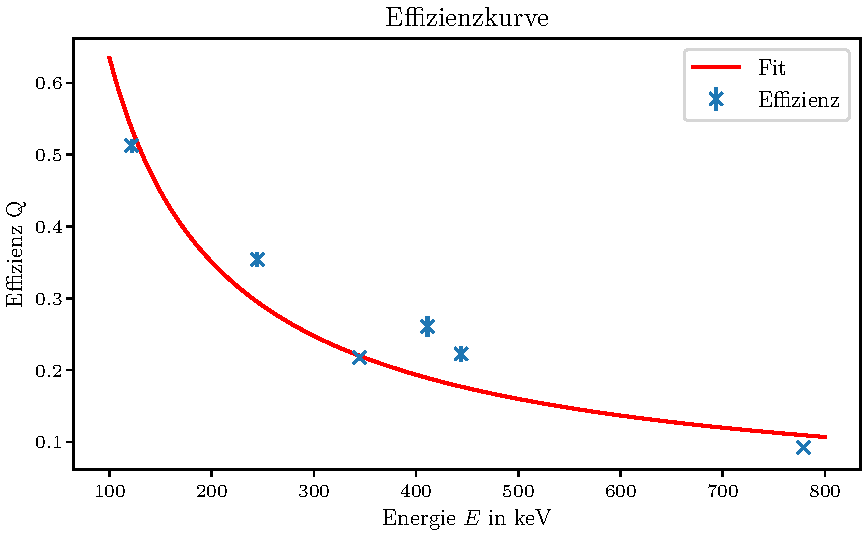
\includegraphics[width=\textwidth]{plots/EuEffizienz.pdf}
    \caption{Effizienz in Abhängigkeit der Energie.}
    \label{fig:effizienz}
\end{figure}

Der Fit ist gegeben durch
\begin{equation}
    Q(E) = \left(\num{32.9(3.0)}\right)\left({\frac{E}{\si{\kilo\electronvolt}}}\right)^{\num{-0.857(16)}}.
    \label{eq:fiteffizienz}
\end{equation}

\subsection{Cäsium-137}

Für Cäsium-137 wird folgendes Spektrum aufgenommen.

\begin{figure}[H]
    \centering
    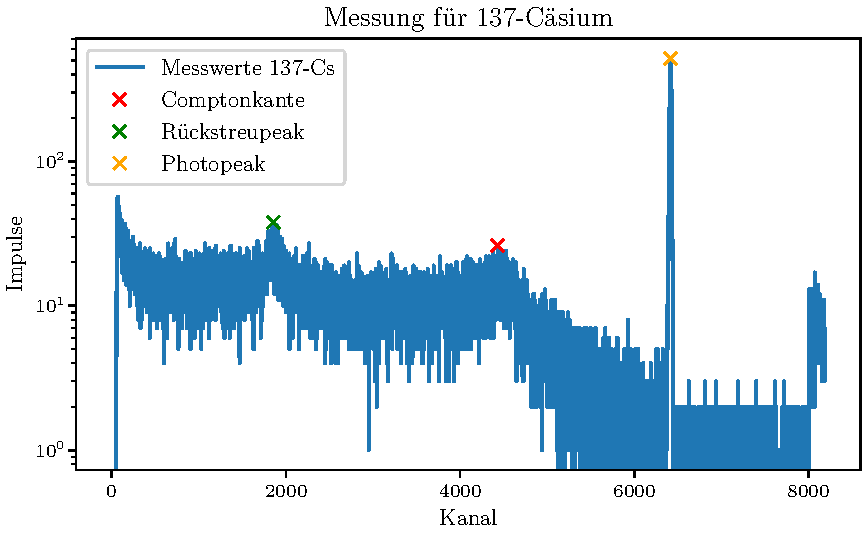
\includegraphics[width=\textwidth]{plots/Caesium.pdf}
    \caption{Die Messung für Cäsium mit ausgewählten, markierten Peaks, vgl. \autoref{tab:LNHB_Cs137}}
    \label{fig:Cäsium}
\end{figure}

Der Photopeak, die Comptonkante und der Rückstreupeak können abgelesen werden. Mit \autoref{eq:E_max} können die letzten beiden Werte auch berechnet werden.
Der Inhalt des Comptonkontinuums, also der Inhalt der Comptonkante in \autoref{tab:fit}, kann über einen Fit des differentiellen Wirkungsquerschnittes \eqref{eq:querschnitt} berechnet werden, zu sehen in \autoref{fig:querschnitt}.
Für die lineare Regression werden die Kanäle 2000 bis 4000 benutzt.

\begin{figure}[H]
    \centering
    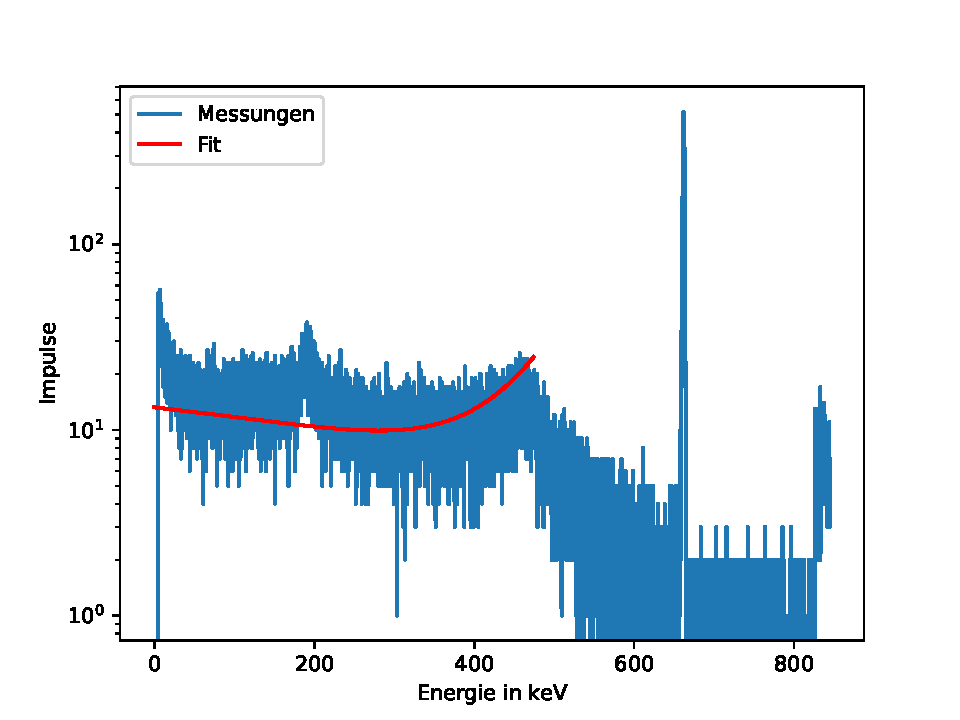
\includegraphics[width=\textwidth]{plots/querschnitt.pdf}
    \caption{Fit des differentiellen Wirkungsquerschnittes. Der Vorfaktor des Fittes berechnet sich zu $\num{6.6185(50)}$.}
    \label{fig:querschnitt}
\end{figure}

Der Vorfaktor $k = \frac{3}{8} \sigma_\text{Th} \frac{1}{m_0 c^2 \epsilon^2}$ berechnet sich hier zu
\begin{equation}
    k = \qty{6.618(5)}{\barn}
\end{equation}

\begin{table}[H]
    \centering
    \caption{Photopeak, Comptonkante, Rückstreupeak}
    \label{tab:fit}
    \begin{tabular}{c c c c c}
        \toprule
        {Name} & {Kanalnr.} & {Energie ($\si{\kilo\electronvolt}$)} & Theoretische Energie ($\si{\kilo\electronvolt}$) & Inhalt \\
        \midrule
        {Photopeak} & 6415 & \num{661(8)} & 661.65 & \num{1176(11)e4} \\
        {Comptonkante} & 4430 & \num{457(7)} & 477 & 12125 \\
        {Rückstreupeak} & 1856 & \num{191(4)} & 184 & {-} \\
        \bottomrule
    \end{tabular}
\end{table}


Für den Photopeak des Cäsium-Spektrum lassen sich für einen Gauß-Fit der Form
\begin{equation}
    f(x) = \frac{a}{\sqrt{2\pi \sigma^2}} \cdot \exp^{-\frac{(x-\mu)^2}{2\sigma^2}}
    \label{eq:gauß}
\end{equation}

folgende Parameter bestimmen.

\begin{align}
    a &= \qty{12233.183(110637)}{\text{Impulse}} \\
    \mu &= \qty{6415.685(89)}{\text{Kanal}} \\
    \sigma &= \qty{9.764(63)}{\text{Kanal}}
\end{align}

\begin{figure}[H]
    \centering
    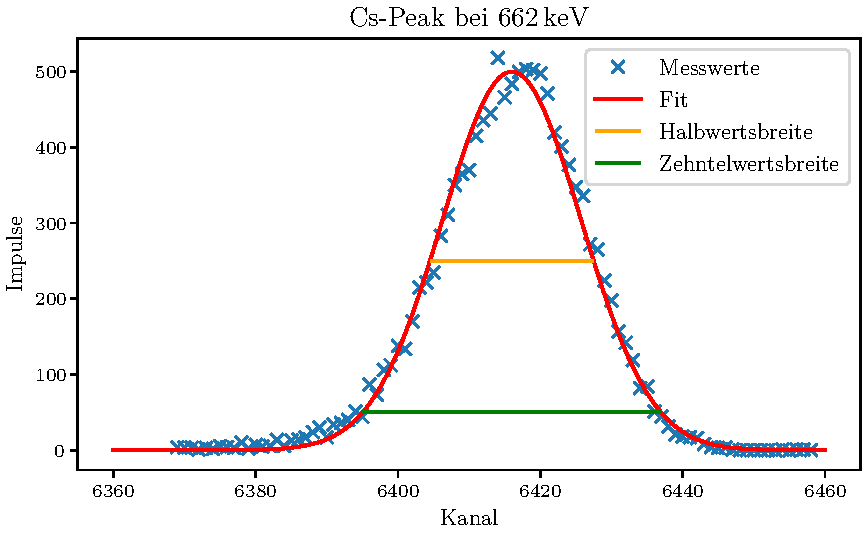
\includegraphics[width=\textwidth]{plots/CsPeak.pdf}
    \caption{Der Cäsium-Peak mit Fit, Halbwerts- und Zehntelwertsbreiten.}
    \label{fig:cspeak}
\end{figure}

Für die Halbwerts- und Zehntelwertsbreiten findt sich
\begin{table}[H]
    \centering
    \caption{Halbwerts- und Zehntelwertsbreiten}
    \label{tab:breiten}
    \begin{tabular}{c c c c}
        \toprule
        {Breite} & {Impulse} & {Breite (Kanäle)} & {Breite ($\si{\kilo\electronvolt}$)} \\
        \midrule
        Halbwertsbreite & 249,89 & 22,922 & $\qty{1.464(188)}{\kilo\electronvolt}$ \\
        Zehntelwertsbreite & 49,978 & 41,841 & $\qty{3.419(188)}{\kilo\electronvolt}$ \\
        \bottomrule
    \end{tabular}
\end{table}

Das Verhältnis von Zehntel- zu Halbwertsbreite $\frac{E_\text{Zehntel}}{E_\text{Halb}}$  einer Normalverteilkung ist konstant und kann zur Überprüfung genutzt werden. Es gilt
\begin{align}
        \frac{E_\text{Zehntel}}{E_\text{Halb}} &\approx  1,823 \\
        \frac{41,841}{22,922} &\approx 1,825
\end{align}

Die Absorptionswahrscheinlichkeiten lassen sich mit Hilfe der Extinktionskoeffizienten % HIER REF ZU BILD
und \eqref{eq:Absorptionswahrscheinlichkeit} berechnen. Die $\mu$ werden dabei dem Altprotokoll \cite{Altprotokoll} entnommen. Die Einschätzung eines sinnvollen Fehlers war nicht möglich.
\begin{align}
    \mu_\text{Photo} &= 0,007 \\
    P_\text{Photo} &= 2,693 \% \\
    \mu_\text{Compton} &= 0,37 \\
    P_\text{Compton} &= 76,37 \%
\end{align}


\subsection{Barium-133}

Für Barium lässt sich folgendes Spektrum aufzeichnen.

\begin{figure}[H]
    \centering
    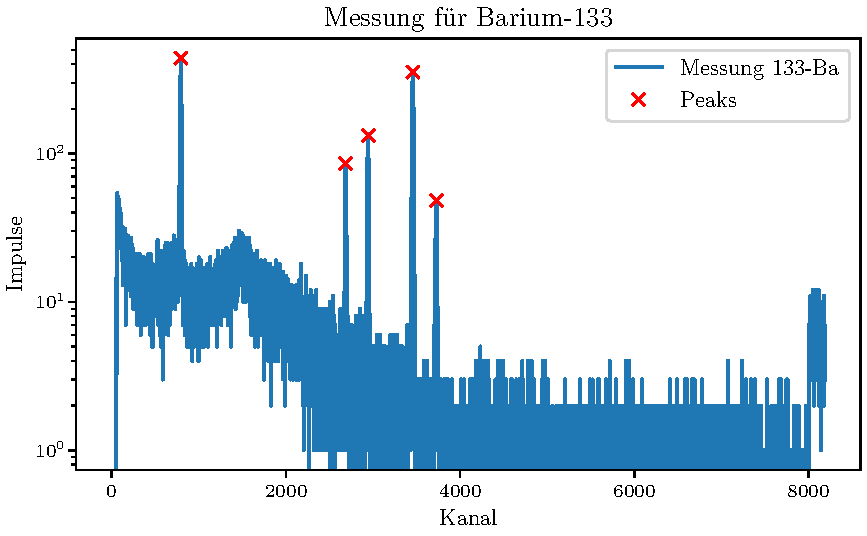
\includegraphics[width=\textwidth]{plots/Barium.pdf}
    \caption{Die Messung von Barium-133 mit ausgewählten, markierten Peaks.}
    \label{fig:barium}
\end{figure}

Die Kanäle, entsprechenden Energien, Wahrscheinlichkeiten und Effizienzen können \autoref{fig:barium} entnommen werden.

\begin{table}[H]
    \centering
    \caption{Kanäle, Energien, Linieninhalte, Wahrscheinlichkeiten und Effizienzen von Barium-133., vgl. \autoref{tab:LNHB_Ba133}}
    \label{tab:barium}
    \begin{tabular}{c c c c c}
        \toprule
        {Kanalnr.} & {Energie ($\si{\kilo\electronvolt})$} & {Inhalt} & {Wahrscheinlichkeit (\%)} & {Q ($\num{1e-3}$)} \\
        \midrule
        793  & \num{81.02(19)}  & \num{6879(33)} & \num{33.31(3)}  & \num{7.60(1)} \\
        2684 & \num{276.37(22)} & \num{1095(33)} & \num{7.13(6)}   & \num{2.65(1)} \\
        2944 & \num{303.23(23)} & \num{2258(47)} & \num{18.31(11)} & \num{2.45(1)} \\
        3456 & \num{356.12(24)} & \num{6183(78)} & \num{62.05(19)} & \num{2.13(1)} \\
        3727 & \num{384.11(25)} & \num{855(29)}  & \num{8.94(6)}   & \num{2.00(1)} \\
        \bottomrule
    \end{tabular}
\end{table}

Die Effizienzen werden dabei mit \eqref{eq:fiteffizienz} berechnet. Mit \eqref{eq:effizienz} 
können Aktivitäten berechnet werden, wobei die Messzeit hier $\qty{3461}{\second}$ lautet. Die mittlere Aktivität ermittelt sich zu
\begin{equation}
    \bar{A}_\text{Ba} = \qty{801(10)}{\becquerel}
\end{equation}

\subsection{Unbekanntes Erz}

Für das unbekannte Erz wird folgendes Spektrum aufgenommen.

\begin{figure}[H]
    \centering
    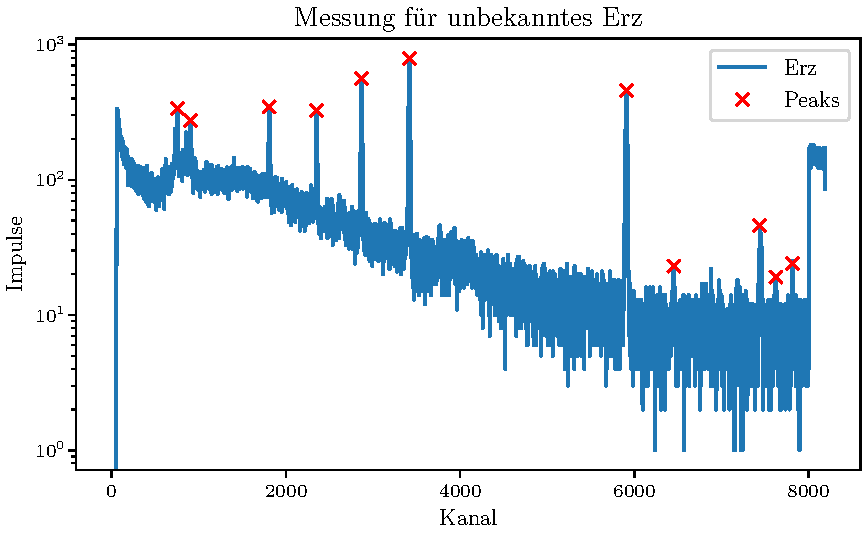
\includegraphics[width=\textwidth]{plots/H.pdf}
    \caption{Spektrum des unbekannten Erzes mit deutlich erkennbaren Peaks.}
    \label{fig:erz}
\end{figure}

\begin{table}[H]
    \centering
    \caption{Kanäle, Energien, Elemente, Linieninhalte, Wahrscheinlichkeiten und Effizienzen vom Erz. \cite{Altprotokoll}}
    \label{tab:erz}
    \begin{tabular}{c c c c c c}
        \toprule
        {Kanalnr.} & {Energie ($\si{\kilo\electronvolt})$} & Element & {Inhalt} & {Wahrscheinlichkeit (\%)} & {Effizienz ($\num{1e-3}$)} \\
        \midrule
        755  & \num{77.09(19)}  & Th & \num{8215(90)}   & \num{3.75(8)}    & \num{7.934(16)} \\
        903  & \num{92.38(19)}  & Th & \num{6982(83)}   & \num{2.18(19)}   & \num{6.794(12)} \\
        1808 & \num{185.87(20)} & Ra & \num{7362(85)}   & \num{3.555(19)}  & \num{3.731(35)} \\
        2351 & \num{241.96(21)} & Pb & \num{6209(78)}   & \num{7.268(22)}  & \num{2.976(22)} \\
        2867 & \num{295.27(22)} & Pb & \num{9925(99)}   & \num{18.414(36)} & \num{2.509(16)} \\
        3417 & \num{352.08(24)} & Pb & \num{15003(122)} & \num{35.6(7)}    & \num{2.157(12)} \\
        5913 & \num{609.93(32)} & Bi & \num{10148(100)} & \num{45.49(19)}  & \num{1.347(60)} \\
        6455 & \num{665.92(34)} & Bi & \num{572(23)}    & \num{1.530(7)}   & \num{1.249(54)} \\
        7442 & \num{767.88(37)} & Bi & \num{1084(32)}   & \num{4.892(16)}  & \num{1.105(46)} \\
        7626 & \num{786.89(38)} & Pb & \num{459(21)}    & \num{1.064(13)}  & \num{1.082(45)} \\
        7818 & \num{806.73(39)} & Bi & \num{520(22)}    & \num{1.262(6)}   & \num{1.060(44)} \\
        \bottomrule
    \end{tabular}
\end{table}

Die berechneten Aktivitäten können folgender Tabelle entnommen werden.

\begin{table}[H]
    \centering
    \caption{Aktivität vom Erz.}
    \label{tab:erz_aktivität}
    \begin{tabular}{c c}
        \toprule
        {Kanalnr.} & {Aktivität ($\si{\becquerel}$)} \\
        \midrule 
        755 & \num{4650(112)} \\
        903 & \num{7940(698)} \\
        1808 & \num{9349(120)} \\
        2351 & \num{4835( 63)} \\
        2867 & \num{3618( 37)} \\
        3417 & \num{3289( 70)} \\
        5913 & \num{2789( 30)} \\
        6455 & \num{5040(212)} \\
        7442 & \num{3375(103)} \\
        7626 & \num{6710(323)} \\
        7818 & \num{6547(288)} \\
        \bottomrule
    \end{tabular}
\end{table}

Da sich die Werte für dieselben Isotope stark unterscheiden, wird auf eine Mittelwertbildung verzichtet.